\subsection{Tasks}
\label{sec:tasks}

Since in SASS-C Verif radar plot coordinates are not given as latitude/longitude, which are the main coordinates for all processing in ATSDB, optionally these coordinates can be re-calculated and set in the database using the ''Calculate Radar Plot Position`` Task.

\subsubsection{Calculate Radar Plot Position}
To execute this task select ''Task``->  ''Calculate Radar Plot Position` in the top menu bar.

\begin{figure}[H]
  \center
    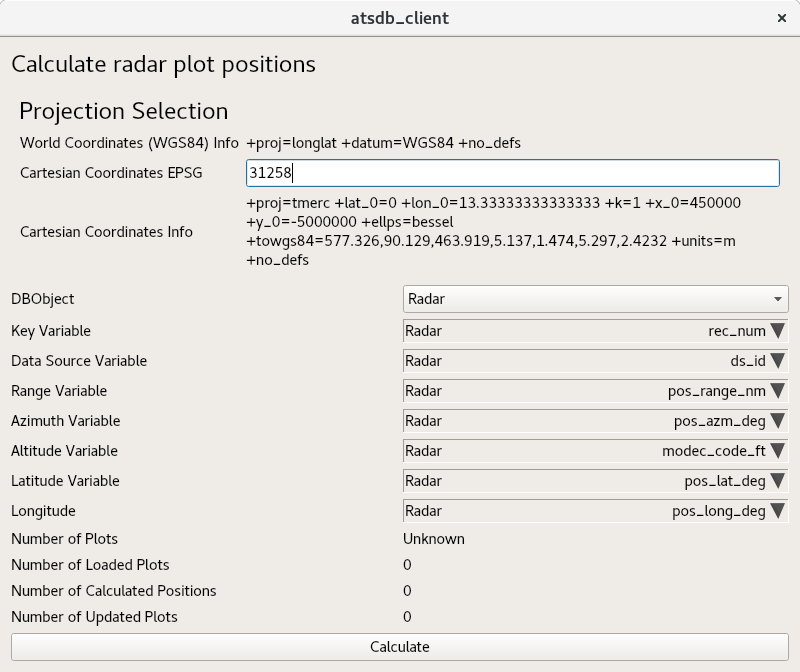
\includegraphics[width=14cm,frame]{../screenshots/task_calc_radar.png}
  \caption{Calculate radar plot position task}
  \label{fig:task_calc_radar}
\end{figure}

The EPSG code for the projection has to be chosen according to your needs, please refer to \url{http://spatialreference.org/ref/epsg/} for a list of possible codes.

The WGS84 latitude/longitude coordinates are then calculated using the radar positions in the database, the range and the azimuth. Press ``Calculate'' to start the calculation process, which will take a few minutes depending on the data size. \\

Please \textbf{note} that currently the various ``Number of'' labels are not set correctly, and no status indication exists. This will be fixed in a later version. \\

Messages like these will be printed in the text console, the last one indicates completion of the task:

\begin{verbatim}
...
[INFO] RadarPlotPositionCalculatorTask: loadingDoneSlot: starting calculation
[INFO] RadarPlotPositionCalculatorTask: loadingDoneSlot: writing update_buffer
[INFO] RadarPlotPositionCalculatorTask: loadingDoneSlot: update_buffer size 7230527
[INFO] RadarPlotPositionCalculatorTask: loadingDoneSlot: end
[INFO] UpdateBufferDBJob: run: start
[INFO] UpdateBufferDBJob: run: writing object Radar key rec_num size 7230527
[INFO] BufferWriter: update: buffer size 7230527 into table sd_radar
[INFO] SQLGenerator: createDBUpdateStringBind: idvar name REC_NUM
[INFO] BufferWriter: update: preparing bind statement
[INFO] BufferWriter: update: starting inserts
[INFO] BufferWriter: update: bind transactions cnt 0
[INFO] BufferWriter: update: bind transactions cnt 100000
...
[INFO] BufferWriter: update: bind transactions cnt 7200000
[INFO] BufferWriter: update: ending bind transactions
UpdateBufferDBJob: run: buffer write done (411.33 s).
\end{verbatim}

After running this task once (per database), the radar plots also have a set latitude/longitude. This task can be re-run with different projections if wanted.
 
